\documentclass{beamer}


\usepackage{tabu}
\usepackage[english]{babel}
\usepackage{algorithm}
\usepackage{algpseudocode}

\usepackage[utf8]{inputenc}

\usepackage[english]{babel}
\usepackage{verbatim}
\usepackage{graphicx}
\usepackage{subcaption}
\usepackage{mwe}
\usepackage{amsmath}
\usepackage{bm}
\usepackage{tikz}
\usepackage{verbatim}
\usepackage{textcomp}
\usetikzlibrary{fit, positioning, shapes,arrows}
\usepackage{multirow}
\usepackage{multicol} % Required for multiple columns
\usepackage{algorithm}
\usepackage{algpseudocode}
\usepackage[utf8]{inputenc}
\usepackage[english]{babel}
\usepackage{appendixnumberbeamer}
\DeclareMathOperator{\EX}{\mathbb{E}}% expected value
\usepackage{graphicx}

\usepackage{hyperref}       % hyperlinkssample-bibliography-biblatex
\usepackage{url}            % simple URL typesetting
\usepackage{booktabs}       % professional-quality tables
\usepackage{amsfonts}       % blackboard math symbols
\usepackage{nicefrac}       % compact symbols for 1/2, etc.
\usepackage{microtype}      % microtypography
\usepackage{algorithm}
\usepackage{bm}


\tikzset{three sided/.style={
        draw=none,
        append after command={
            [shorten <= -0.5\pgflinewidth]
            ([shift={(-1.5\pgflinewidth,-0.5\pgflinewidth)}]\tikzlastnode.north east)
        edge([shift={( 0.5\pgflinewidth,-0.5\pgflinewidth)}]\tikzlastnode.north west) 
            ([shift={( 0.5\pgflinewidth,-0.5\pgflinewidth)}]\tikzlastnode.north west)
        edge([shift={( 0.5\pgflinewidth,+0.5\pgflinewidth)}]\tikzlastnode.south west)            
            ([shift={( 0.5\pgflinewidth,+0.5\pgflinewidth)}]\tikzlastnode.south west)
        edge([shift={(-1.0\pgflinewidth,+0.5\pgflinewidth)}]\tikzlastnode.south east)
        }
    }
}

\makeatletter
\DeclareRobustCommand{\rchi}{{\mathpalette\irchi\relax}}
\newcommand{\irchi}[2]{\raisebox{\depth}{$#1\chi$}} 

\newcommand*\bigcdot{\mathpalette\bigcdot@{.5}}
\newcommand*\bigcdot@[2]{\mathbin{\vcenter{\hbox{\scalebox{#2}{$\m@th#1\bullet$}}}}}
\makeatother



% to compile a camera-ready version, add the [final] option, e.g.:
% \usepackage[final]{nips_2016}

\usepackage{nicefrac}       % compact symbols for 1/2, etc.
\usepackage{microtype}      % microtypography
\setbeamerfont{caption}{series=\normalfont,size=\fontsize{6}{6}} 
\usepackage{breakcites}
\usepackage[tableposition=top]{caption}

\usepackage{ragged2e}
\usepackage{etoolbox}
\usepackage{lipsum}


\apptocmd{\frame}{}{\justifying}{} % Allow optional arguments after frame.

\colorlet{Mycolor1}{green!10!orange!90!}
\definecolor{foreground}{RGB}{255,255,255}
\definecolor{background}{RGB}{30,30,30}
\definecolor{title}{RGB}{107,174,214}
\definecolor{gray}{RGB}{155,155,155}
\definecolor{subtitle}{RGB}{102,255,204}
\definecolor{hilight}{RGB}{102,255,204}
\definecolor{vhilight}{RGB}{255,111,207}
\definecolor{footline}{RGB}{255,255,255}

\setbeamercolor{titlelike}{fg=title}
\setbeamercolor{subtitle}{fg=subtitle}
\setbeamercolor{institute}{fg=gray}
\setbeamercolor{normal text}{fg=foreground,bg=background}

\usepackage{lipsum}

\defbeamertemplate{headline}{page number}{%
	\vskip1pt%
	\setbeamertemplate{footline}[page number]%
	\usebeamertemplate{footline}%
}
\setbeamertemplate{headline}[page number]
\setbeamercolor{page number in head/foot}{fg=white}



\usepackage[absolute,overlay]{textpos}

\mode<presentation>
{
  \usetheme{default}      % or try Darmstadt, Madrid, Warsaw, ...
  \usecolortheme{default} % or try albatross, beaver, crane, ...
  \usefonttheme{default}  % or try serif, structurebold, ...
  \setbeamertemplate{navigation symbols}{}
  \setbeamertemplate{caption}[numbered]
} 
\usepackage{acronym}

%%Theo's stuff
\newcommand{\theo}[1]{{\color{blue}Theo: [#1]}}
\newcommand{\edwin}[1]{{\color{green}Edwin: [#1]}}
\newcommand{\virginia}[1]{{\color{red}Virginia: [#1]}}

% abbreviations
\newcommand{\etal}{et al.\xspace}
\newcommand{\ie}{i.e.\xspace}
\newcommand{\eg}{e.g.\xspace}
\newcommand{\Ie}{I.e.\xspace}
\newcommand{\eq}{Eq.\xspace}
\newcommand{\eqs}{Eqs.\xspace}
\newcommand{\fig}{Fig.\xspace}
\newcommand{\secref}[1]{\S \ref{#1}}
\newcommand{\iid}{i.i.d.~\xspace}
\newcommand{\dgp}{DGP\xspace}
\newcommand{\tbl}{Tab.\xspace}


% Acronyms
\newcommand{\supplement}{supplement}
\newcommand{\acro}[1]{\textsc{#1}\xspace}
\newcommand{\lgcp}{\acro{lgcp}}
\newcommand{\icm}{\acro{icm}}
\newcommand{\lgcpn}{\acro{lgcpn}}
\newcommand{\lgcpnnormal}{\acro{lgcpn-n}}
\newcommand{\lgcpngp}{\acro{lgcpn-gp}}
\newcommand{\mlgcp}{\acro{mlgcp}}
\newcommand{\pool}{\acro{pooling}}
\newcommand{\lgcpc}{\acro{lgcp-c}}
\newcommand{\lgcpnc}{\acro{lgcpn-c}}
\newcommand{\gptext}{\acro{gp}}
\newcommand{\mtl}{\acro{mtl}}
\newcommand{\stl}{\acro{stl}}
\newcommand{\mcmc}{\acro{mcmc}}
\newcommand{\mala}{\acro{mala}}
\newcommand{\inla}{\acro{inla}}
\newcommand{\lcm}{\acro{lcm}}
\newcommand{\rbf}{\acro{rbf}}
\newcommand{\btb}{\acro{btb}}
\newcommand{\gt}{\acro{gt}}
\newcommand{\mv}{\acro{mv}}
\newcommand{\nypd}{\acro{nypd}}
\newcommand{\nlpl}{\acro{nlpl}}
\newcommand{\rmse}{\acro{rmse}}
\newcommand{\crime}{\acro{crime}}
\newcommand{\cpu}{\acro{cpu}}
\newcommand{\gb}{\acro{gb}}
\newcommand{\ram}{\acro{ram}}


% Matrices and vectors 
\newcommand{\mat}[1]{\mathbf{#1}}
\renewcommand{\vec}[1]{ \mathbf{#1} } % math bold
\newcommand{\vecS}[1]{\boldsymbol{ #1 }  } % this for boldsymbols
\newcommand{\vecentry}[2]{{\mathrm #1_{#2}}}
\newcommand{\matentry}[3]{{\mathrm #1_{#2,#3}}}
\newcommand{\matcol}[2]{\mat{#1}_{\cdot,#2}}
\newcommand{\matrow}[2]{\mat{#1}_{#2,\cdot}}

% GP things
\newcommand{\gp}{\mathcal{GP}}
\newcommand{\kernel}{\kappa}
\newcommand{\meanfunc}[1]{m(#1)}
\newcommand{\covfunc}[3]{\kernel(#1,#2; #3)}
\newcommand{\hyperparam}{\vectheta}

% Specific variables
\newcommand{\dataset}{\mathcal{D}}
\newcommand{\x}{\vec{x}}
\newcommand{\xn}{\x_n}
\newcommand{\xstar}{\x_\star}
\newcommand{\xprime}{\x^{\prime}}
\newcommand{\vectheta}{\vecS{\theta}}
\newcommand{\y}{\vec{y}}
\newcommand{\ystar}{\y_\star}
\newcommand{\yn}{\vec{y}_n}
\newcommand{\f}{\mat{F}}
\newcommand{\fstar}{\f_\star}
%\newcommand{\u}{\vec{u}}
\newcommand{\fq}{\f_{\bullet q}}
\newcommand{\fn}{\f_{n \bullet}}
\newcommand{\samplefn}[1]{\fn^{(#1)}}
\newcommand{\W}{\mat{W}}
\renewcommand{\wp}{\W_{p \bullet}}
\newcommand{\varw}{\sigma^2} % variance of W for independent prior
\newcommand{\wq}{\W_{\bullet q}}
\newcommand{\samplewp}[1]{\wp^{(#1)}}
\newcommand{\Y}{\mat{Y}}
\newcommand{\lambdan}{\vec{\lambda}_{n \bullet}}
\renewcommand{\u}{\mat{U}}
\newcommand{\uq}{\u_{\bullet q}}
\newcommand{\z}{\vec{z}}
\newcommand{\Z}{\mat{Z}}
\newcommand{\Zq}{\Z_q}
\newcommand{\zprime}{\z^{\prime}}
\newcommand{\meanfu}{\tilde{\vecS{\mu}}}  % conditonal prior mean
\newcommand{\covfu}{\widetilde{\vecS{\mat{K}}}}  % conditonal prior covariance
\newcommand{\meanfuq}{\tilde{\vecS{\mu}}_q}  % conditonal prior mean
\newcommand{\covfuq}{\widetilde{\vecS{\mat{K}}}_q}  % conditonal prior covariance
\newcommand{\likeparam}{\phi}

% Covariance matricces
\newcommand{\Kq}{\mat{K}_{xx}^q}
\newcommand{\covwq}{\vecS{\mat{K}}_{w}^q}
\newcommand{\Kzzq}{\mat{K}_{zz}^q}
\newcommand{\Kxzq}{\mat{K}_{xz}^q}
\newcommand{\Kzxq}{\mat{K}_{zx}^q}
\newcommand{\Kzzqinv}{(\mat{K}_{zz}^q)^{-1}}


% Distributions
\newcommand{\poisson}{\text{Poisson}}
\newcommand{\normal}{\mathcal{N}}

% statistics / algebra / computation
\newcommand{\kl}[2]{\mathrm{KL}(#1 \lVert #2)}
\newcommand{\expectation}[2]{ \mathbb{E}_{#1}{\left[#2\right]} }
\renewcommand{\det}[1]{\left\lvert#1\right\rvert}
\newcommand{\trace}{\mbox{ \rm tr }}
\newcommand{\bigO}{\mathcal{O}}

% variational stuff
\newcommand{\varparam}{\vecS{\nu}}
\newcommand{\varmeanuq}{\vec{m}_q}
\newcommand{\varmeanfqn}{\mu_q}
\newcommand{\varmeanfq}{\pmb{\mu}_q}
\newcommand{\varcovuq}{\mat{S}_q}
\newcommand{\varmeanwq}{\vecS{\omega}_q}
\newcommand{\varmeanwpq}{\omega_{pq}}
\newcommand{\varcovwq}{\vecS{\Omega}_q}
\newcommand{\varcovwpq}{\Omega_{pq}}
\newcommand{\varcovfq}{\Sigma^q}
\newcommand{\varvarwq}{\tilde{\sigma}^2_q}
\newcommand{\calL}{\mathcal{L}}
\newcommand{\elbo}{\calL_{\text{elbo}}}
\newcommand{\ellterm}{\calL_{\text{ell}}}
\newcommand{\klterm}{\calL_{\text{kl}}}
\newcommand{\enterm}{\calL_{\text{ent}}}
\newcommand{\crossterm}{\calL_{\text{cross}}}
\newcommand{\elltermhat}{\widehat{\calL}_{\text{ell}}}  
\newcommand{\qfn}{q(\fn) }
\newcommand{\qwp}{q(\wp)}





\title[]{Constrained Bayesian Optimisation with Knowledge Gradient}
\author[Juan Ungredda]{\small Juan Ungredda}
\institute[]{University of Warwick}
\date{}


\begin{document}


\begin{frame}
  \titlepage
  \flushright
\includegraphics[ height=0.8cm]{logo_epsrc.jpeg}
  
\includegraphics[ height=0.8cm]{logo_warwick.jpeg}
\end{frame}


\section{Background}

\begin{frame}{Constrained KG}
Non-constrained KG:
$$KG(x) = \mathbb{E}[\max_{x'}\{\mu^{n+1}(x')\}|x^{n+1}=x]$$

Constrained KG with Probability of Feasibility (pf):
\begin{align*}
\begin{split}
cKG(x) &= \mathbb{E}[\max_{x'}\{pf^{n+1}(x')\mu^{n+1}(x')\}|x^{n+1}=x]
\end{split}
\end{align*}

Constrained KG corrected*:
\begin{align*}
\begin{split}
cKG(x) &= \mathbb{E}[\max_{x'}\{pf^{n+1}(x')\mu^{n+1}(x') + (1-pf^{n+1}(x'))M\}|x^{n+1}=x]
\end{split}
\end{align*}

where $M\in \mathbb{R}$ is the penalisation for sampling points in an infeasible region. It's commonly assumed to be zero.

\end{frame}

\begin{frame}{Constrained KG}
Benefits
\begin{itemize}
	\item Takes into account that constraints change for each possible $x^{n+1}$ considered.
	\item Assuming $M=0$ may give "benefit" to infeasible regions. A more general approach avoids that problem.
\end{itemize}
Limitations
\begin{itemize}
	\item Computationally expensive compared to constrained Expected Improvement. However, it's possible to make an efficient implementation by using gradients.
	\item $M$ may be need to chosen by the decision maker.
\end{itemize}

\end{frame}

\begin{frame}{Results}
benchmark Method:
\begin{itemize}
	\item Constrained Expected Improvement. i.e. Expected Improvement times Probability of feasibility. 
\end{itemize}
Test Functions:
\begin{itemize}
	\item New Branin, test function 2, and Mistery function. Non-noisy and Noisy objective functions with unknown constraints.
\end{itemize}

Important Remark:
\begin{itemize}
	\item In the last evaluation of our approach, the function is sampled according to Expected Improvement times the probability of feasibility.
\end{itemize}

\end{frame}

\begin{frame}{Performance Evaluation}
Given sampled data $D^{N} = \{(x_{0},y_{0}),\dots, (x_{N},y_{N}) \}$. The recommended design is given by the max value of the Gaussian Process approximation $\mu^{N}$.

$$
x_{r} = \max_{D^{N}}\mu^{N}(x)
$$


Performance is measured as difference in true value $y_{true}$ (if it's noisy) between best true design $x^{*}$ and recommended sampled design $(x_{r})$.

$$
Performance(x_{r}) = y_{true}(x_{r}) - y_{true}(x_{r}) 
$$

For real experiments performance was measured as
$$
Performance(x_{r}) = y_{true}(x_{r}) 
$$

\end{frame}


\begin{frame}{PLOTS}
\begin{figure}
	
	\centering
	\begin{tabular}{ccc}
		Mistery&
		New Branin&
		Test function 2\\
		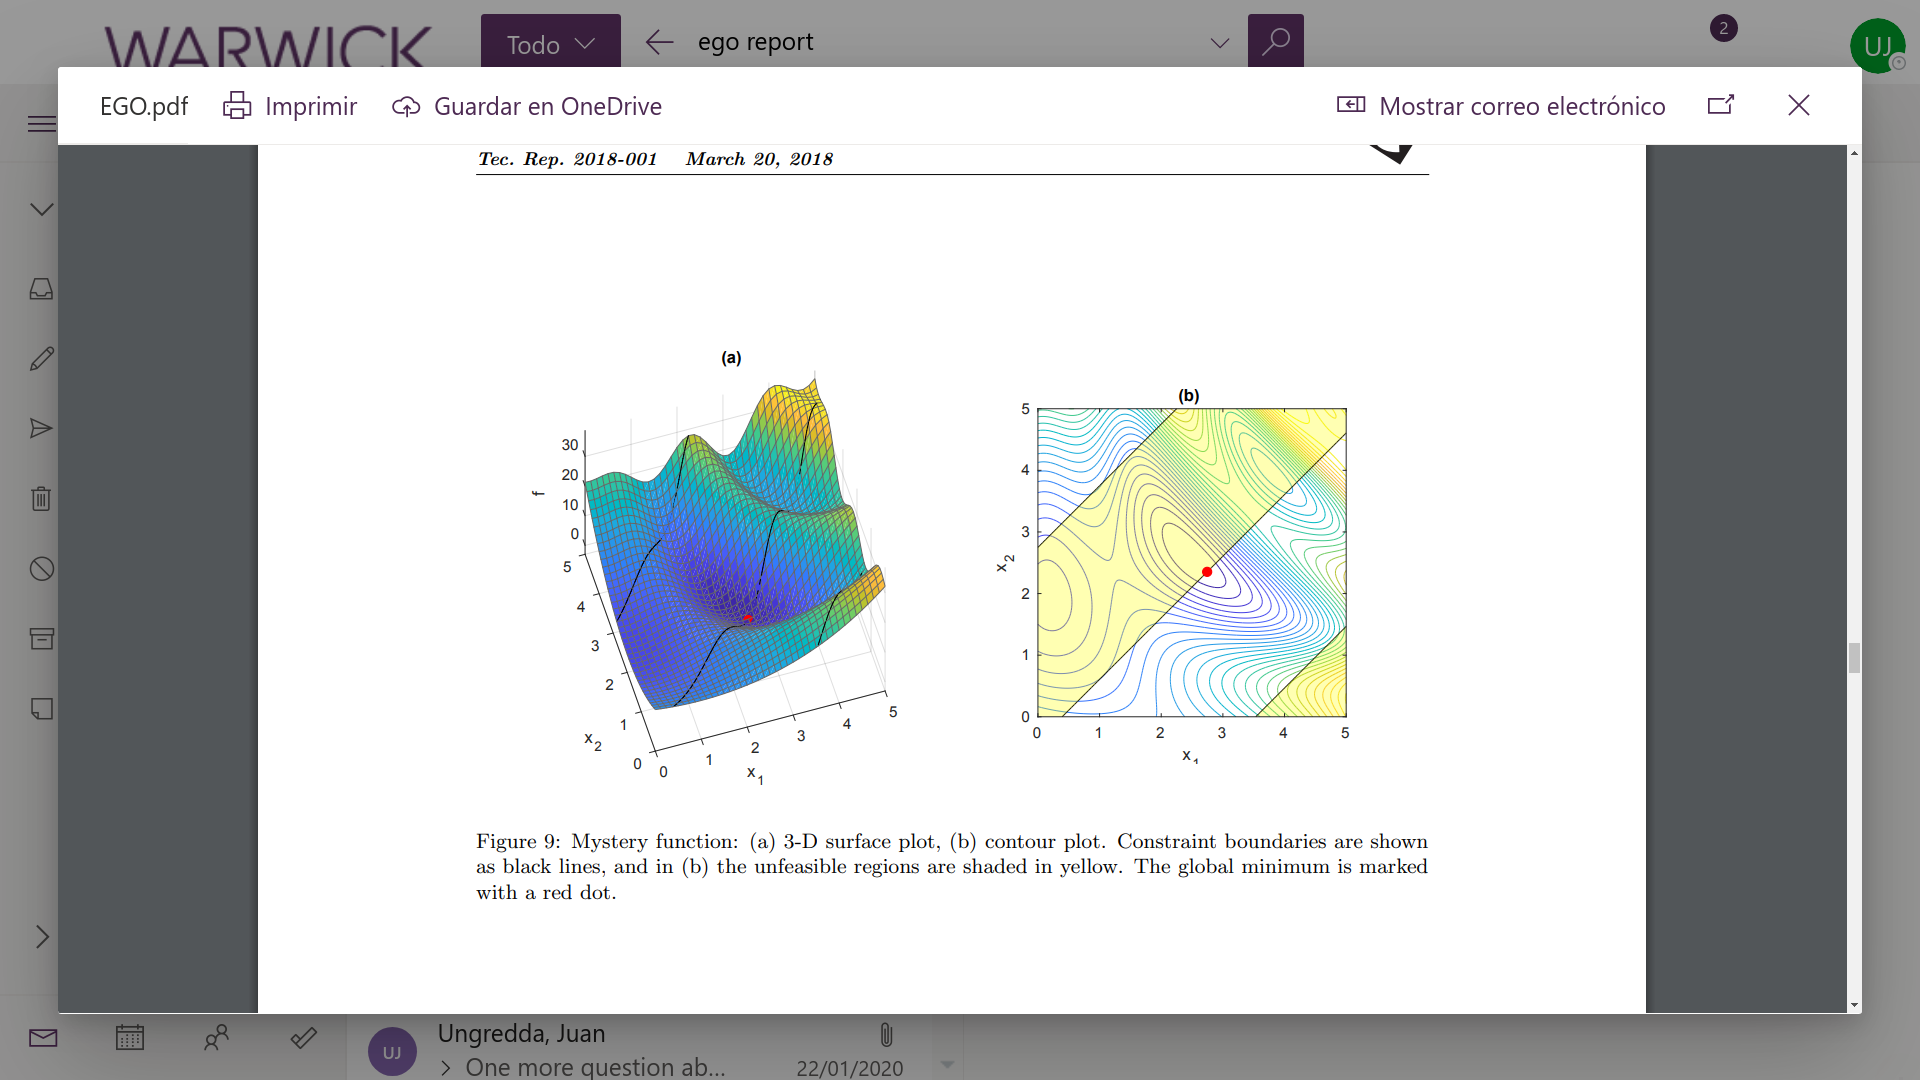
\includegraphics[height=1.6cm, trim={450 300 450 300},clip]{Mistery.png}&
		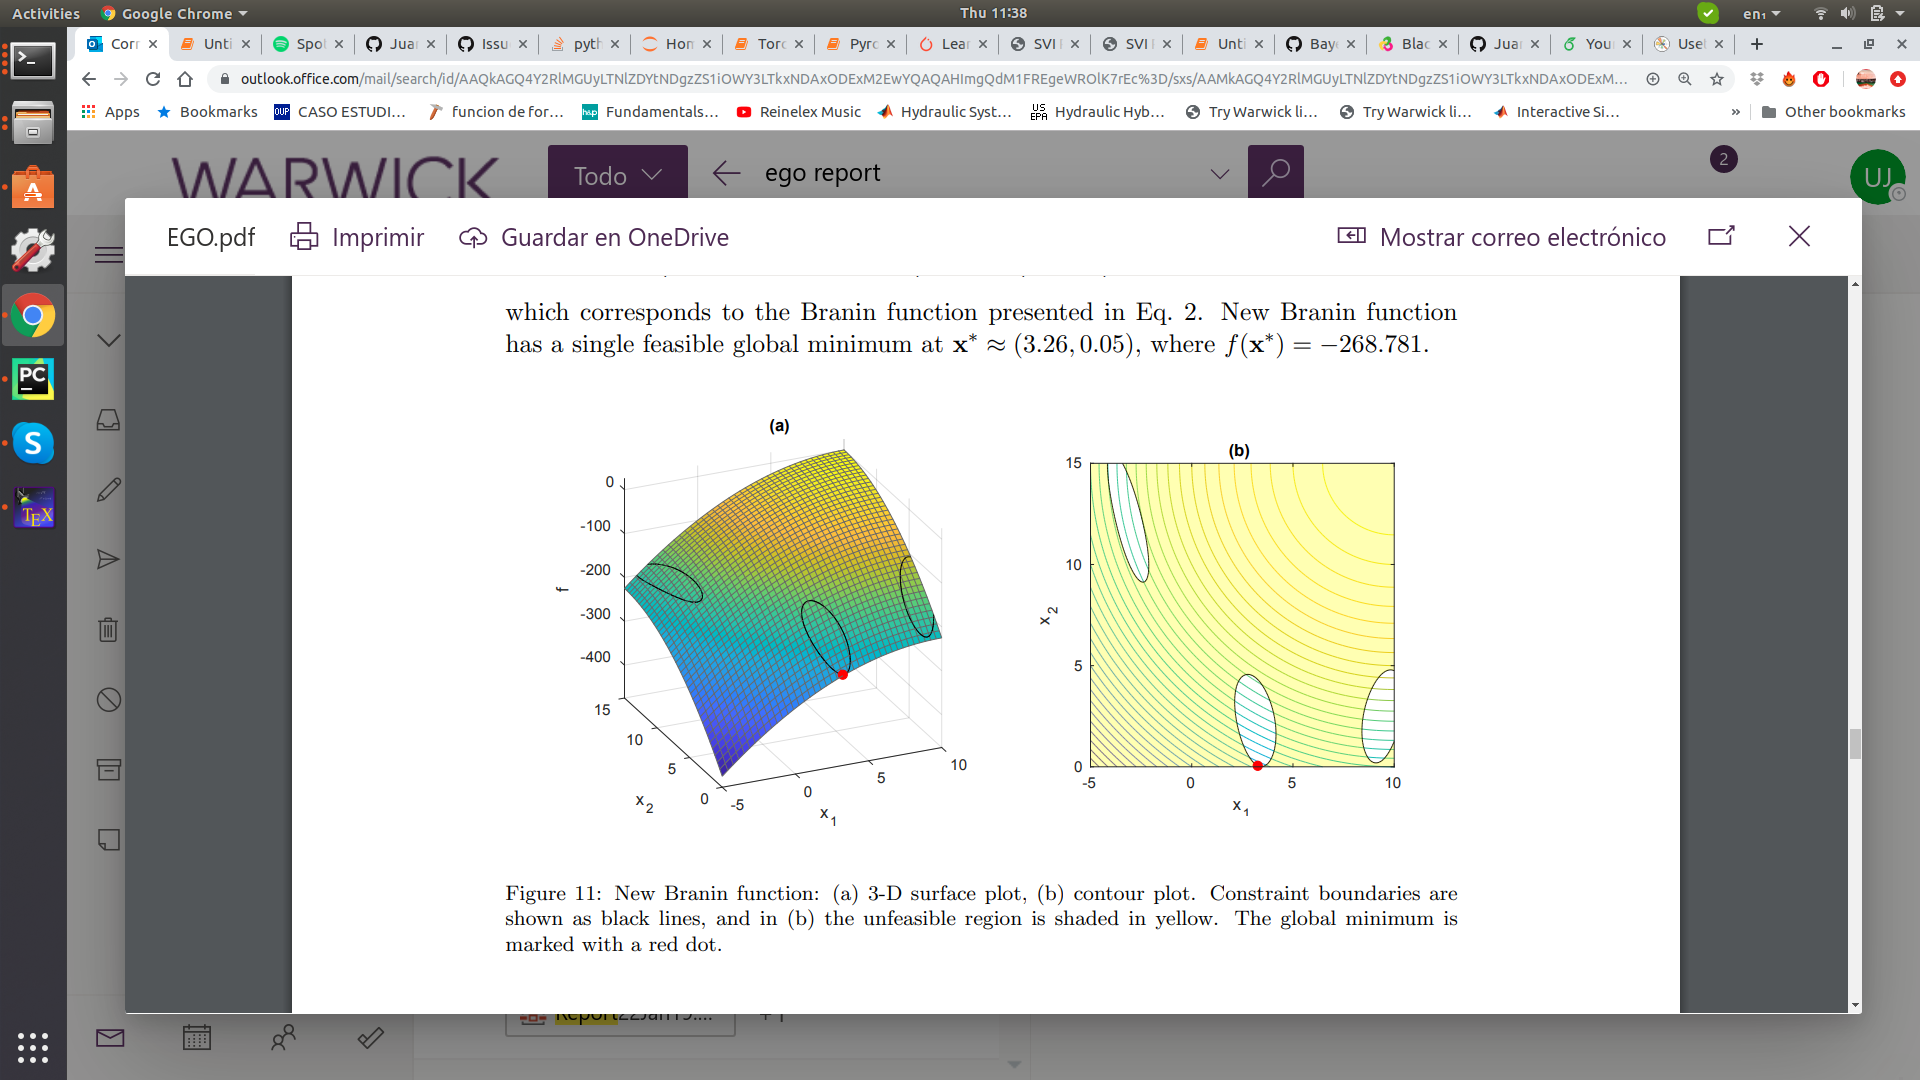
\includegraphics[height=1.6cm, trim={450 240 450 360},clip]{New_Branin.png}&
		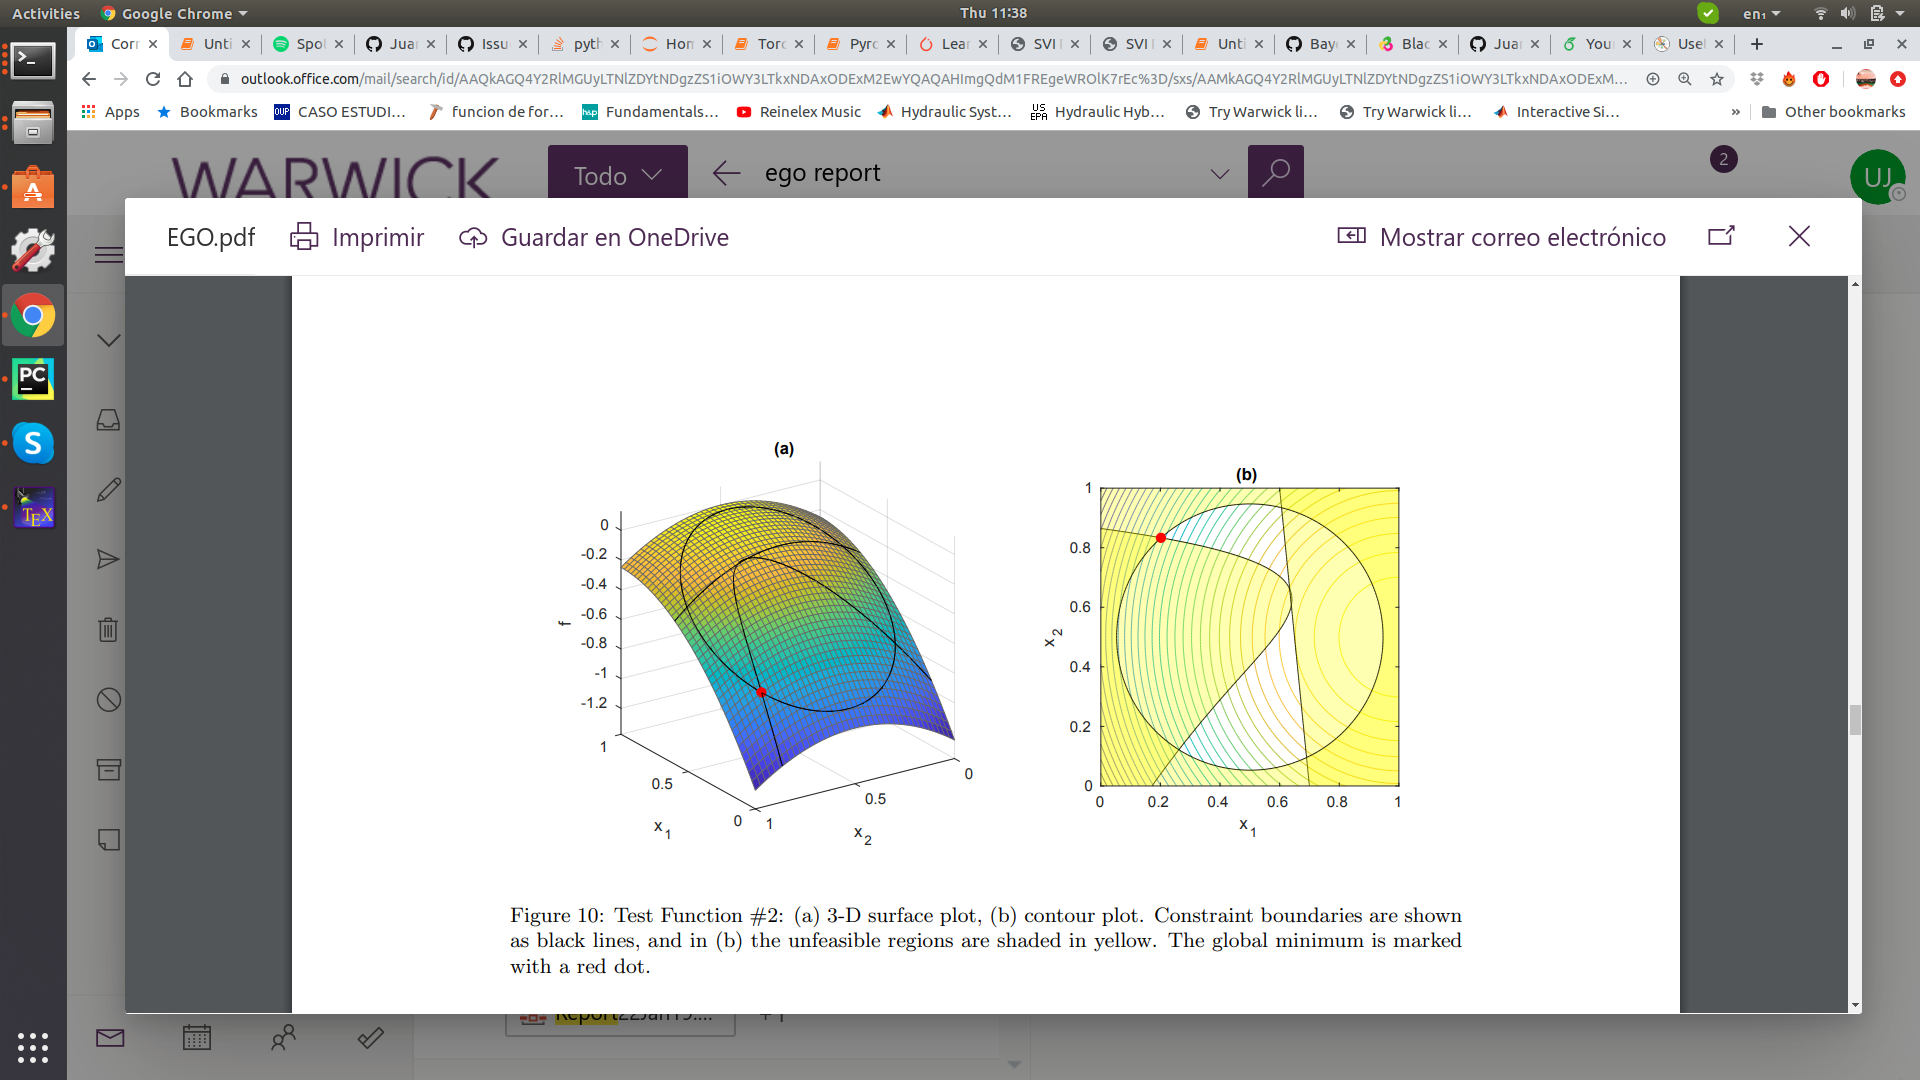
\includegraphics[height=1.6cm, trim={450 230 450 370},clip]{test_function_2.png}\\
		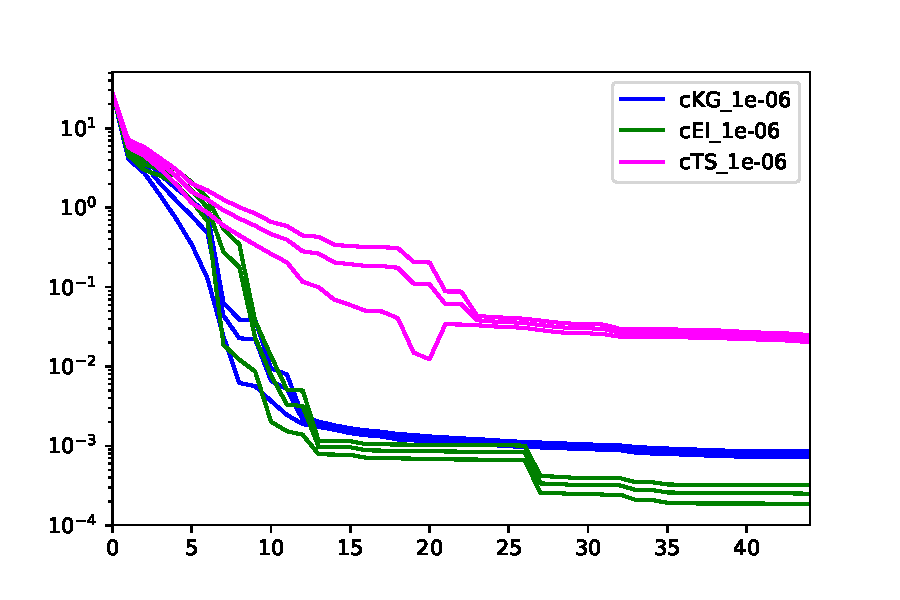
\includegraphics[width=0.32\linewidth]{mistery_OC_1e-06.pdf}&
		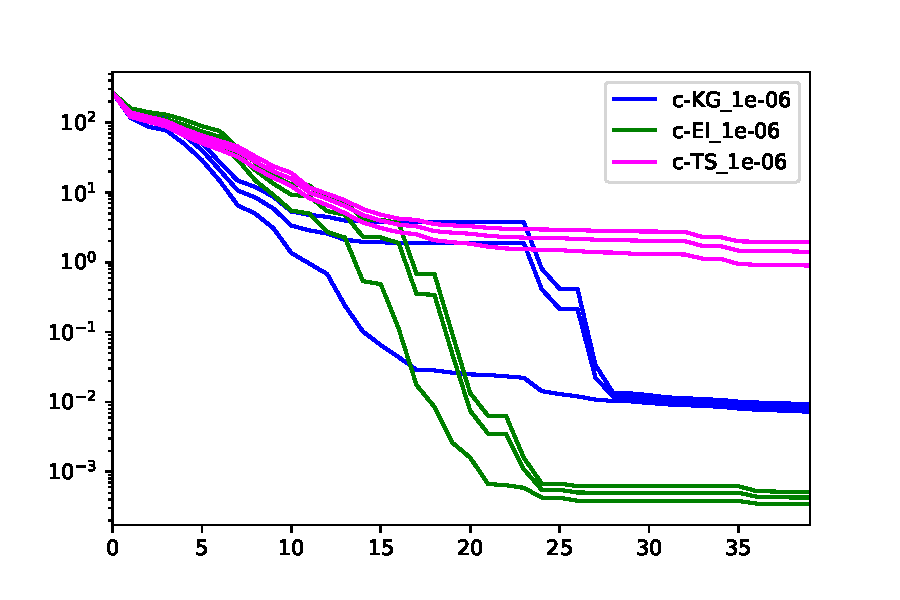
\includegraphics[width=0.32\linewidth]{new_brannin_OC_1e-06.pdf}&
		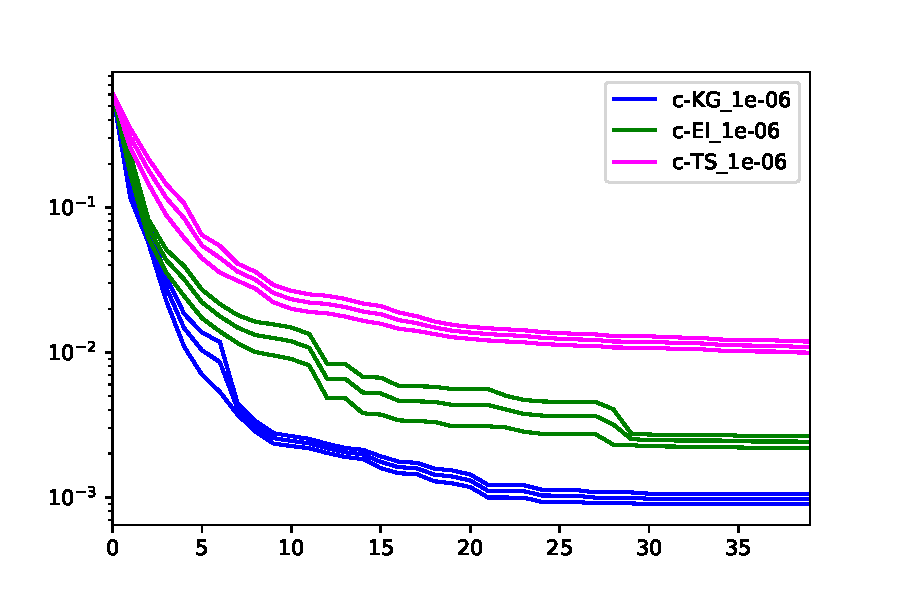
\includegraphics[width=0.32\linewidth]{test_function_OC_1e-06.pdf}\\
		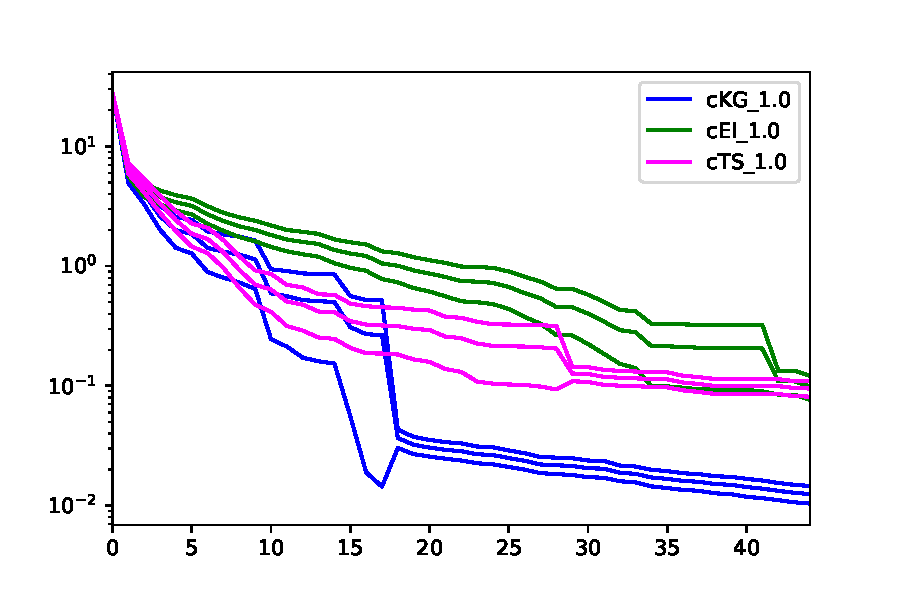
\includegraphics[width=0.32\linewidth]{mistery_OC_1_0.pdf}&
		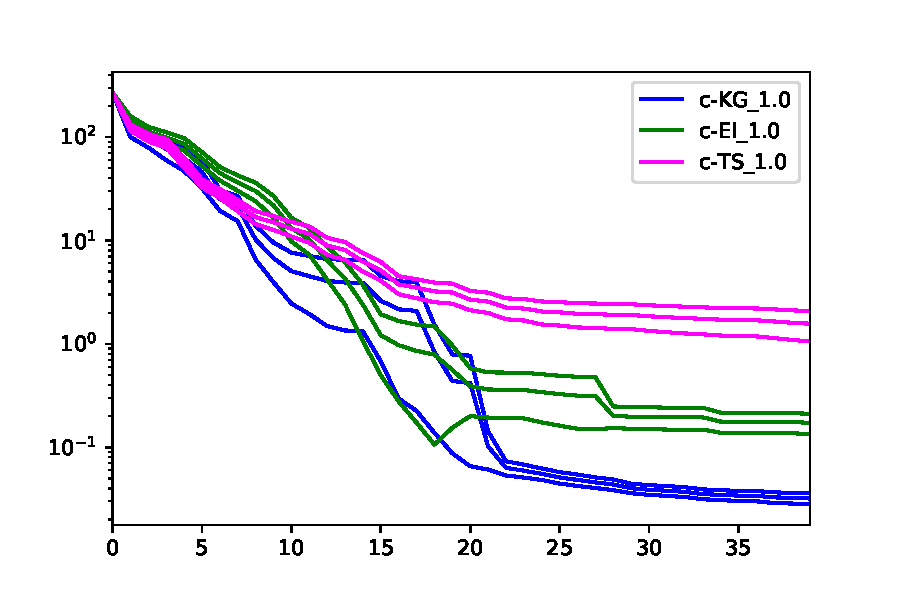
\includegraphics[width=0.32\linewidth]{new_brannin_OC_1_0.pdf}&
		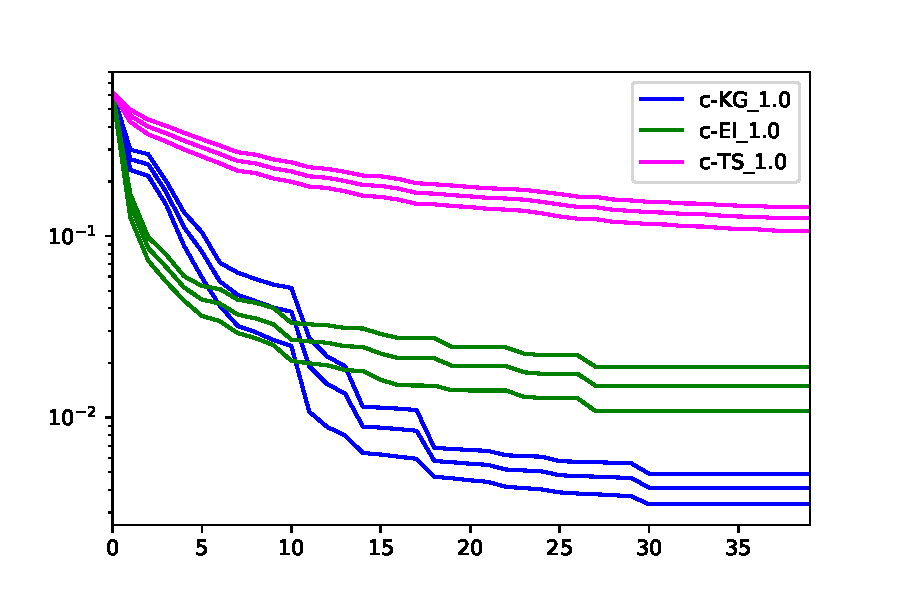
\includegraphics[width=0.32\linewidth]{test_function_OC_1_0.pdf}\\
	\end{tabular}	
\end{figure}
\end{frame}


\begin{frame}{Real Experiments (Multi-Stage Revenue Management with Inter-Temporal Dependence)}

A businessman chooses to buy b > 0 units of capacity, paying c > 0 dollars per unit of capacity at $t = 0$.During stage $t (t = 1, \dots , T)$ he observes demand $D_{t}$ for units at price $p_{t}$, at which point, he must choose to sell $x_{t}$ units $(0 \leq xt \leq D_{t})$, provided that the total number of units sold (accross all past periods) does not exceed b.

\begin{figure}
	
	\centering
	\begin{tabular}{c}
		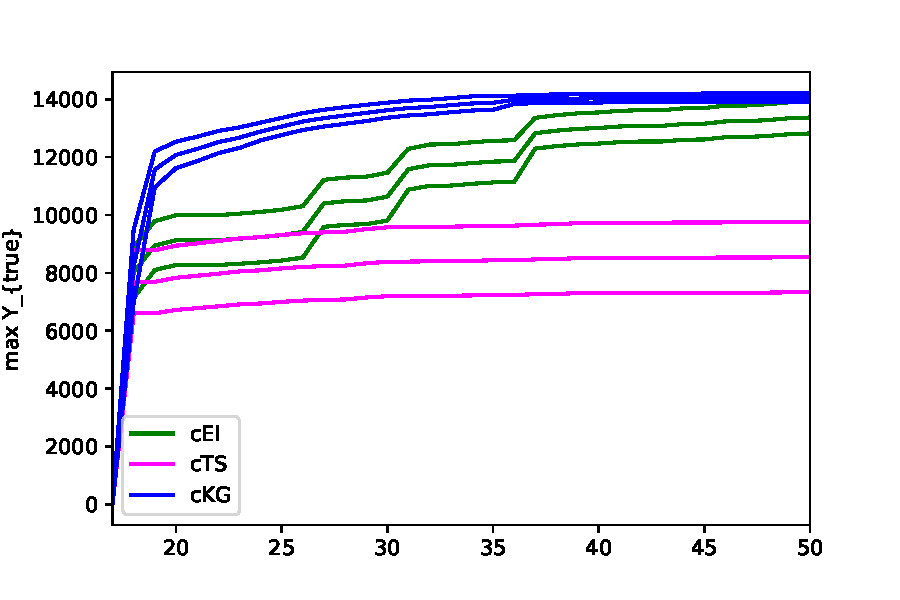
\includegraphics[width=0.7\linewidth]{RMITD_OC.pdf}\\
	\end{tabular}	
\end{figure}
\end{frame}

\begin{frame}{Real Experiments (Tuning a Fully Connected Neural Network)}

I tune the hyperparamters of a two-hidden-layer neural network subject to
the constraint that the prediction time must not exceed 0.01s. The search space consists of 4 parameters: 2 dropout parameters, and the number of hidden units in each layer.

\begin{figure}
	
	\centering
	\begin{tabular}{c}
		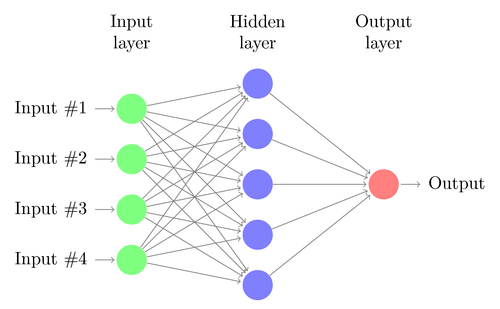
\includegraphics[width=0.7\linewidth]{FC_NN.png}\\
	\end{tabular}	
\end{figure}
\end{frame}




\begin{frame}{Gradient Information}

\begin{itemize}
	\item Numerical methods to optimise KG rely on $\nabla$KG. Quantity can be obtained either by Finite Difference or Analytically. 
\end{itemize}

\begin{align*}
\begin{split}
\nabla cKG(x) &= \nabla \mathbb{E}[\max_{x'}\{pf^{n+1}(x')\mu^{n+1}(x')\}|x^{n+1}=x]
\end{split}
\end{align*}

Once solved, the inner optimisation problem, 

\begin{align*}
\begin{split}
\nabla cKG(x) &= \mathbb{E}[\nabla \{pf^{n+1}(x^{*};x^{n+1})\mu^{n+1}(x^{*};x^{n+1})\}|x^{n+1}=x]
\end{split}
\end{align*}

Potential issue with Finite Differences:
\begin{itemize}
	\item Since the expectations is calculated only over a few values slight deviations of $x^{*}$ affect greatly the outer gradient estimation. 
\end{itemize}

\end{frame}
	

\begin{frame}{Dynamically change of M penalization.}

\begin{figure}
	
	\centering
	\begin{tabular}{ccc}
		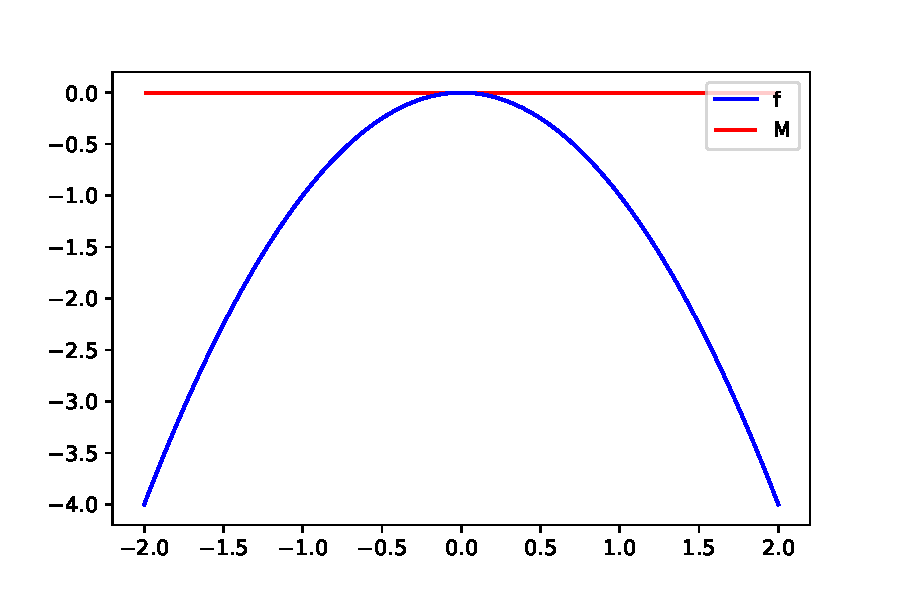
\includegraphics[width=0.32\linewidth]{penalty_image0.pdf}&
		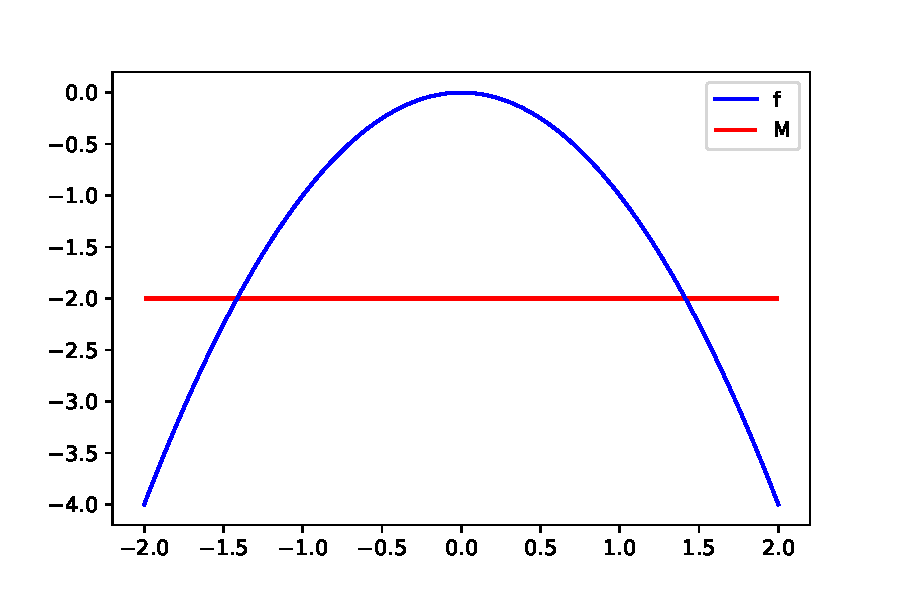
\includegraphics[width=0.32\linewidth]{penalty_image-2.pdf}&
		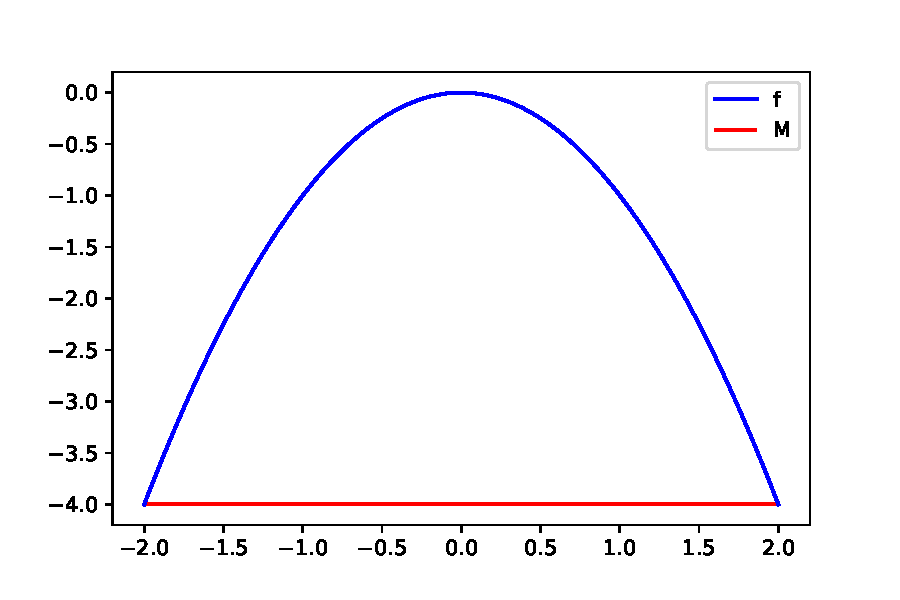
\includegraphics[width=0.32\linewidth]{penalty_image-4.pdf}\\
		(a)&
		(b)&
		(c)\\
		
	\end{tabular}	
\end{figure}
\end{frame}

\begin{frame}{Dynamically change of M penalization (Formulation)}

\begin{align*}
\begin{split}
cKG(x) &= \mathbb{E}[\max_{x'}\{pf^{n+1}(x')\mu^{n+1}(x') + (1-pf^{n+1}(x'))M\}|x^{n+1}=x]
\end{split}
\end{align*}

$$
M = (\mu(x) - \mu^{*}) \sum_{i}{\mu_{c_{i}}(x)}
$$
\begin{itemize}
	\item $(\mu(x) - \mu^{*})$ penalises values with higher negative values $\mu(x)$ far from estimated optimum $\mu^{*})$
	\item $\sum_{i}{\mu_{c_{i}}(x)}$ penalises regions far from feasible area.
\end{itemize}
\end{frame}

\begin{frame}{Result plots}

Constrained Brannin function using dynamic change of penalisation on EGO. Comparison against highly penalised infeasibility (M=-999), and encouraged infeasibility (M=2).

\begin{figure}
	
	\centering
	\begin{tabular}{cc}
		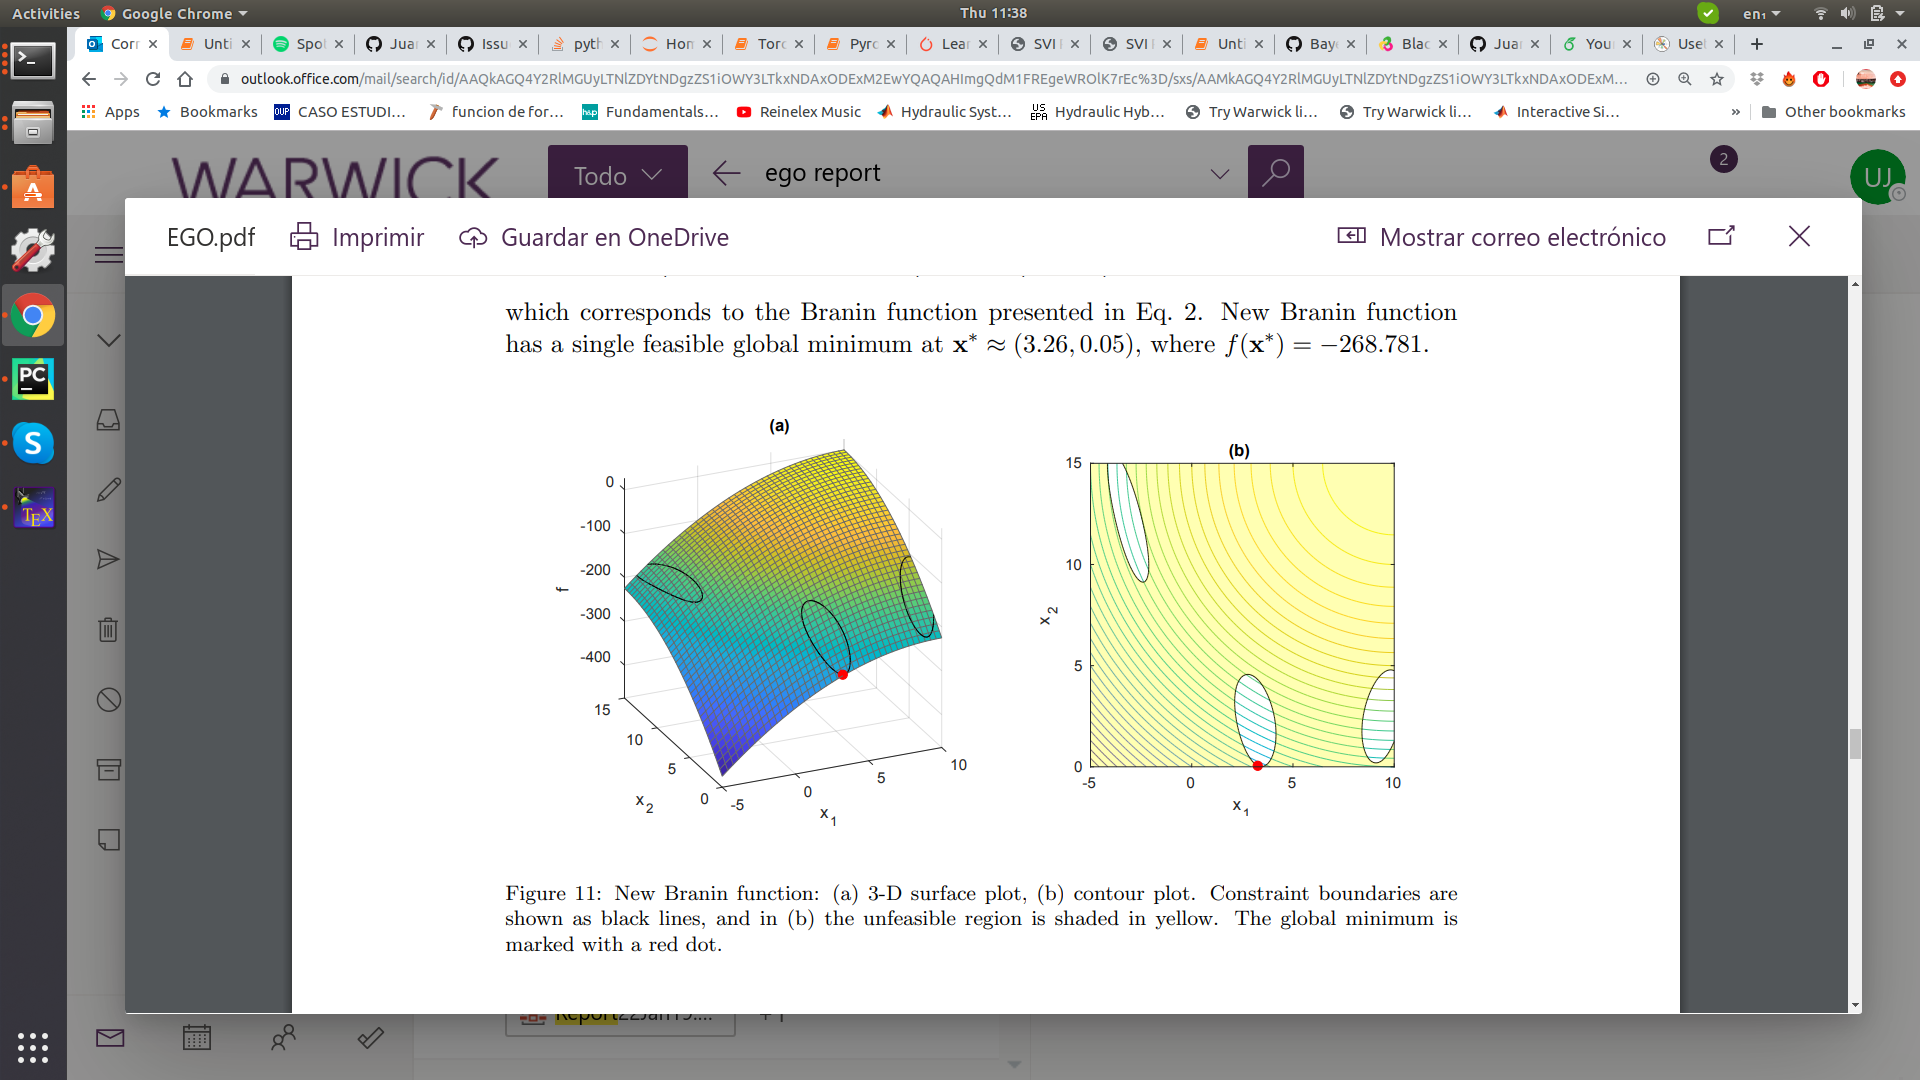
\includegraphics[height=2.6cm, trim={450 240 450 360},clip]{New_Branin.png}&
		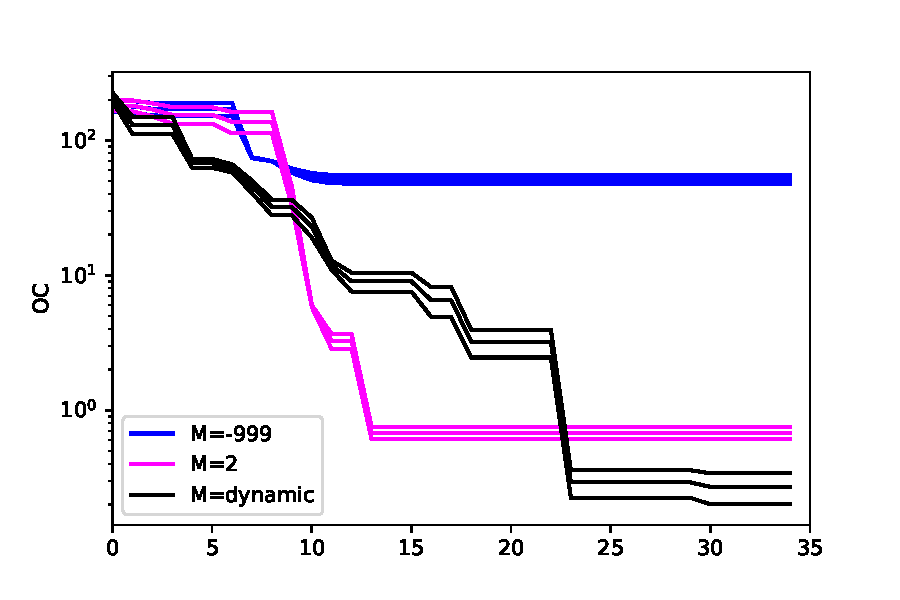
\includegraphics[width=0.5\linewidth]{penalty_OC.pdf}\\

	\end{tabular}	
\end{figure}

\end{frame}

\begin{frame}{Multi-Objective Constrained Optimisation}

\begin{itemize}
	\item Multi-Objective formulation using linear scalarisation.
\end{itemize}

$$
KG(x';\theta) = \mathbb{E}_{y}[\max_{x'}\theta\mu^{n+1}(x')|x^{n+1}=x',\theta]
$$
where the policy is,
$$
maKG(x') = \mathbb{E}_{\theta}[KG(x';\theta)]
$$

\begin{itemize}
	\item Multi-Objective constrained formulation
\end{itemize}

$$
KG(x';\theta) = \mathbb{E}_{y}[\max_{x'}\theta\mu^{n+1}(x')pf^{n+1}(x')|x^{n+1}=x',\theta]
$$
where the policy is,
$$
maKG(x') = \mathbb{E}_{\theta}[KG(x';\theta)]
$$


\end{frame}






\begin{frame}{Work to do}

Main line of work
\begin{itemize}
	\item Constrained Multi-Objective problem
\end{itemize}

\end{frame}

\end{document}